\section{Redegøre for principperne i .NET frameworket og dets overordnede arkitektur samt beskrive og anvende programmeringssproget C\#}\label{sec:spm1}

\subsection{Hvad er .NET}
% Skal omkring!!
%% CLR runtime thing...
%% Intermediete language, som clr oversætter...

.NET er ef framework udviklet af Microsoft. Programmer som skrives til .NET køres i et virtuelt miljø, kaldet Common Langauge Runtime. CLR er et virtuelt miljø der står for sikkerhed, memory management og exception handling. Kode skrevet med .NET kaldes derfor for \textbf{\textit{Managed Code}} .NET frameworket tillader flere proggrammeringssprog at tale sammen (Language Interoperability).


\subsection{Principper i .NET frameworket}

\begin{itemize}
	\item Interoperability
	\item Language independance - .NET introducerer \textit{Common Type System} som definerer alle de datatyper og construct, som CLR supporterer samt hvordan de interagerer med hinanden. På denne måde yder .NET support udveksling af typer og objekter mellem forskellige libraries og applikationer, så længe de er skrevet i et .NET sprog. 
	\item Portability - .NET er lavet så det er platform uafhængigt. Dog har Microsoft aldrig implementeret hele frameworket på andet end Windows. Microsoft har dog udgivet specifikationerne til Common Intermediate Langage, CIL.
	\item Security - Code Access Security bruges til at forhindre "untrusted code" i at udføre priviledged actions. Når CLR'en loader en assembly fil, identificeres den \textit{gruppe} som koden hører til. En gruppe har et sæt af permissions. Når et stykke kode forøger at udføre en priviligeret handling, kigger CLR'en de permissions som koden har. Disse group permission set er defineret af system aministratoren.
	\item Memory Management/Garbage collection - Se afsnit om garbage collectoren. Hvis en permission ikke gives af CLR'en kastes en security exception.
	\item Performance - Når en applikation køres, kompileres IL koden af en JIT compiler, som cacher programmet i en .NET Native Image Cache. Den næste gang programmet køres er det allerede cachet og indlæses derfor hurtigere.
\end{itemize}

\subsection{Garbage Collection}
Også kendt som \textbf{Managed Heap}. I de \textit{gode gamle dage} var den samme dans nødvendig hver gang en ressource skulle bruges:

\begin{enumerate}
	\item \textbf{Allocate} memory for resource (new operator).
	\item \textbf{Initialize} memory to make resource usable (constructor).
	\item Use the resource (acces members) - repeat as necessary.
	\item \textbf{Tear-down} the resource (destructor).
	\item Free the memory.
\end{enumerate}

Dette fører typisk til nogle almindelige problemer, såsom \textbf{memory leaks} og \textbf{memory corruption}\footnote{Når hukommelse bruges efter frigivelse.}. Dette er seriøse problemer fordi \textit{timing} og \textit{consequence} er uforudsigelige (meget svært at debugge).

\subsubsection{Enter Mr. Garbage Collector} 
Et object \textit{frigives} aldrig i kode. GC\footnote{Garbage Collector} frigiver objecter når de ikke længere er tilgængelige (\textit{reachable}).

\begin{figure}[h]
	\centering
	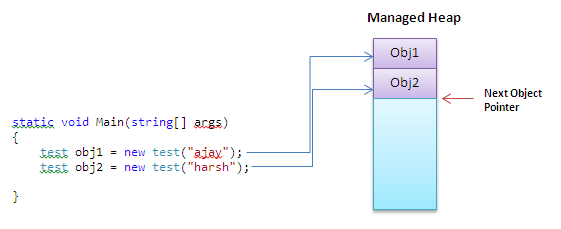
\includegraphics[width=\linewidth]{figs/nextobjptr}
	\caption{Garbage collector's \textit{NextObjectPointer}.}
	\label{fig:nextobjptr}
\end{figure}

\paragraph{Allokering}
\begin{itemize}
	\item Hver process har sin egen virtuelle address space region.
	\item GC sker concurrent, bag om ryggen på os.
	\item Allokering sker i enden af heapen, ved \textit{NextObjPtr} se figur~\ref{fig:nextobjptr}. Hvilket gør denne allokering meget hurtigere end \textit{unmanaged} \textit{new/malloc/HeapAlloc}.
	\item Større objekter\footnote{Over 85KB, kan ændres af microsoft.} allokeres på en speciel heap.
\end{itemize}

\paragraph{Collection ''Mark and Compact''}
\begin{enumerate}
	\item \textbf{Marking}\\
	Objekter som kan \textit{nås} bliver markeret (kaldet \textit{Roots}).
	\item \textbf{Compacting}\\
	Markerede objekter bliver \textit{shifted} ned over de umarkerede.
	\item Hvis alle objekter er markerede forekommer der ikke nogen compacting. Hvis der ikke er mere hukommelse bliver en \textit{OutOfMemoryException} smidt.
\end{enumerate}

\subparagraph{Marking phase}
\begin{itemize}
	\item Marks objects reachable from roots.
	\begin{itemize}
			\item En Root er en memory location, som kan referere til et object, eller være \textit{null}.			
			\begin{itemize}
				\item Static fields defined within a type.
				\item Arguments passed to a method.
				\item Local variables declared within a method.
				\item CPU registers (enrigistered fields, argumenter or variables).
			\end{itemize}			
			\item Roots are always reference types (never value types).
			\item Each method has a root table (produced by JIT compiler).
	\end{itemize}	
	\item Each marked object has its fields checked; these objects are marked too (recursively).
	\item GC walks up the thread's call stack, determining roots for the calling methods by accessing each method's root table (hvor allerede markerede objekter 'skippes').
	\begin{itemize}
		\item Improves performance.
		\item Prevents infinite loops due to circular  references.
		\item Static fields are checked; these objects are marked too.
	\end{itemize}
\end{itemize}

\begin{figure}[h]
\centering
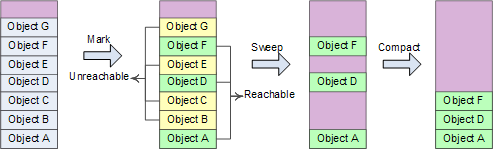
\includegraphics[width=0.8\linewidth]{figs/markandsweep}
\caption{Mark and Compact ved Garbage collection.}
\label{fig:markandsweep}
\end{figure}

\subparagraph{Compacting phase}
\begin{itemize}
	\item Compacts marked objects.
	\begin{itemize}
		\item Marked objects are shifted down (simple memory copy).		
	\end{itemize}
	\item No address space fragmentation unlike the unmanaged heap!
	\begin{itemize}
		\item Each root is updated to point to object's new memory address.
	\end{itemize}
	\item After compacting the heap...
	\begin{itemize}
		\item The \textit{NextObjPtr} pointer is positioned after last surviving object.
		\item The 'new operation that caused the GC is tried again.
		\item Heap should have free space \& new should succed.
	\end{itemize}
	\begin{itemize}
		\item If not, a \textit{OutOfMemoryException} is thrown.
	\end{itemize}
\end{itemize}

\subsection{C\# compiler}
% hvad laver den

\subsection{Assembly}
En assmebly er kompileret kode. Der er to typer:
\begin{itemize}
	\item Process assemblies - .EXE filer. Repræsenterer en process der bruger klasser der er defineret i library assemblies. Assemblies indeholder kode i Intermediate Language.
	\item Library assemblies - .DLL filer.
	Assemblies kompileres til maskinkode af JIT compileren. JIT compileren er en del af CLR
\end{itemize}

\subsection{Overordnet arkitektur i .NET}

\subsection{Anvendelse af C\#}